\chapter{Validaci�n y An�lisis de Resultados} %\index{Validaci�n}

A continuaci�n se muestran un conjunto de simulaciones din�micas realizadas en \textbf{Simulink} para analizar la efectividad de los diferentes esquemas de control definidos en la secci�n \ref{sec:Controlador-Capitulo-2}. Las primeras tres simulaciones se realizan con el fin de comparar los diferentes controladores, mientras que las �ltimas dos tienen el fin de mostrar la efectividad del MCCE en el caso del rodamiento h�brido. 

\section{Controlador retroalimentado y controlador integral} 

Esta simulaci�n consiste en un controlador retroalimentado \ref{fig:esquema-controlador-retroalimentado} y un controlador integral \ref{fig:esquema-controlador-integral}, ambos con un observador de estado y en tiempo continuo. 

Esta simulaci�n se realiza sin cargas externas y con las condiciones iniciales:

\begin{table}[H]
\centering
\begin{tabular}{|l|l|l|l|l|l|l|l|l|l|}
\hline
$x_c$     & $y_c$      & $z_c$     & $\dot{x}_c$     & $\dot{y}_c$     & $\dot{z}_c$     & $\phi$       & $\theta$    & $\dot{\phi}$     & $\dot{\theta}$   \\ \hline
$0.25 mm$ & $-0.25 mm$ & $0.25 mm$ & $0\frac{mm}{s}$ & $0\frac{mm}{s}$ & $0\frac{mm}{s}$ & $-0.0015rad$ & $0.0015rad$ & $0\frac{rad}{s}$ & $0\frac{rad}{s}$ \\ \hline
\end{tabular}
\caption{Condiciones Iniciales: Controlador retroalimentado y Controlador integral.}
\end{table}

\begin{figure}[H]
    \centering
    \begin{subfigure}[b]{0.45\textwidth}
        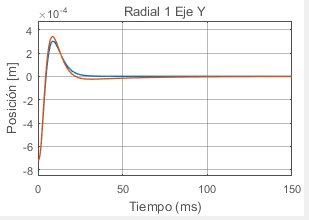
\includegraphics[width=\textwidth]{images/Capitulo_4/retroalimentado_vs_integral/radial_1_eje_y}
        \caption{Radial $1$.}
        %\label{fig:rmr:diagrama-de-polos}
    \end{subfigure}
    ~ %add desired spacing between images, e. g. ~, \quad, \qquad, \hfill etc. 
      %(or a blank line to force the subfigure onto a new line)
    \begin{subfigure}[b]{0.45\textwidth}
        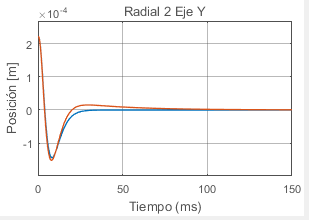
\includegraphics[width=\textwidth]{images/Capitulo_4/retroalimentado_vs_integral/radial_2_eje_y}
        \caption{Radial $2$.}
        %\label{fig:rmr:diagrama-de-fuerzas}
    \end{subfigure}
    \caption{Salida del sistema: Eje $Y$. Control retroalimentado (azul) y control integral (rojo).}
    \label{fig:Controlador_retroalimentado_vs_Controlador_integral_Eje_Y_radial}
\end{figure}

\begin{figure}[H]
    \centering
    \begin{subfigure}[b]{0.45\textwidth}
        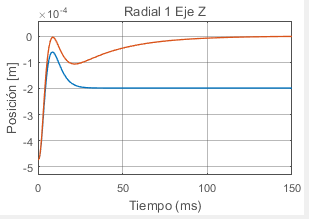
\includegraphics[width=\textwidth]{images/Capitulo_4/retroalimentado_vs_integral/radial_1_eje_z}
        \caption{Radial $1$.}
        %\label{fig:rmr:diagrama-de-polos}
    \end{subfigure}
    ~ %add desired spacing between images, e. g. ~, \quad, \qquad, \hfill etc. 
      %(or a blank line to force the subfigure onto a new line)
    \begin{subfigure}[b]{0.45\textwidth}
        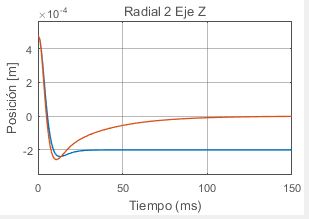
\includegraphics[width=\textwidth]{images/Capitulo_4/retroalimentado_vs_integral/radial_2_eje_z}
        \caption{Radial $2$.}
        %\label{fig:rmr:diagrama-de-fuerzas}
    \end{subfigure}
    \caption{Salida del sistema: Eje $Z$. Control retroalimentado (azul) y control integral (rojo).}
    \label{fig:Controlador_retroalimentado_vs_Controlador_integral_Eje_Z_radial}
\end{figure}

\begin{figure}[H]
    \centering
    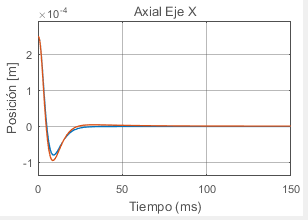
\includegraphics[width=0.45\textwidth]{images/Capitulo_4/retroalimentado_vs_integral/axial_eje_x}
    \caption{Salida del sistema: Eje axial $X$. Control retroalimentado (azul) y control integral (rojo).}
    \label{fig:Controlador_retroalimentado_vs_Controlador_integral_Eje_X_axial}
\end{figure}

La salida del sistema simulado, mostrado en las figuras \ref{fig:Controlador_retroalimentado_vs_Controlador_integral_Eje_Y_radial}, \ref{fig:Controlador_retroalimentado_vs_Controlador_integral_Eje_Z_radial} y \ref{fig:Controlador_retroalimentado_vs_Controlador_integral_Eje_X_axial}, representa el desplazamiento del eje medido desde los extremos del rotor. Podemos observar que ambos controladores llegan a estabilizar la posici�n del eje, sin embargo, el sistema con controlador retroalimentado no converge en la posici�n deseada ($0$), en cambio el sistema con controlador integral s� lo hace.

\newpage

\section{Controlador continuo y controlador discreto} 

Esta simulaci�n consiste en un controlador integral continuo \ref{fig:esquema-controlador-integral} con observador de estados,  y sus versiones discretizadas \ref{fig:esquema-controlador-discreto} el cual opera con una frecuencia de muestreo de $10kHz$. Esta simulaci�n se realiza sin cargas externas y con las condiciones iniciales:

\begin{table}[htb]
\centering
\begin{tabular}{|l|l|l|l|l|l|l|l|l|l|}
\hline
$x_c$     & $y_c$      & $z_c$     & $\dot{x}_c$     & $\dot{y}_c$     & $\dot{z}_c$     & $\phi$       & $\theta$    & $\dot{\phi}$     & $\dot{\theta}$   \\ \hline
$0.25 mm$ & $-0.25 mm$ & $0.25 mm$ & $0\frac{mm}{s}$ & $0\frac{mm}{s}$ & $0\frac{mm}{s}$ & $-0.0015rad$ & $0.0015rad$ & $0\frac{rad}{s}$ & $0\frac{rad}{s}$ \\ \hline
\end{tabular}
\caption{Condiciones Iniciales: Controlador continuo y Controlador discreto.}
\end{table}

\begin{figure}[htb]
    \centering
    \begin{subfigure}[b]{0.45\textwidth}
        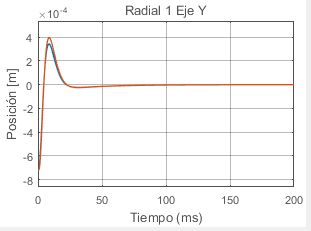
\includegraphics[width=\textwidth]{images/Capitulo_4/continuo_vs_discreto/radial_1_eje_y}
        \caption{Radial $1$.}
        %\label{fig:rmr:diagrama-de-polos}
    \end{subfigure}
    ~ %add desired spacing between images, e. g. ~, \quad, \qquad, \hfill etc. 
      %(or a blank line to force the subfigure onto a new line)
    \begin{subfigure}[b]{0.45\textwidth}
        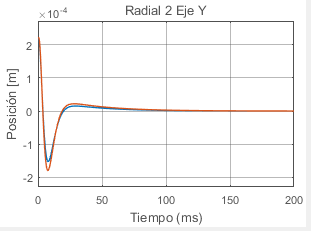
\includegraphics[width=\textwidth]{images/Capitulo_4/continuo_vs_discreto/radial_2_eje_y}
        \caption{Radial $2$.}
        %\label{fig:rmr:diagrama-de-fuerzas}
    \end{subfigure}
    \caption{Salida del sistema: Eje $Y$. Control integral continuo (azul) y control integral discreto (rojo).}
    \label{fig:Controlador_continuo_vs_Controlador_discreto_Eje_Y}
\end{figure}

\newpage

\begin{figure}[H]
    \centering
    \begin{subfigure}[b]{0.45\textwidth}
        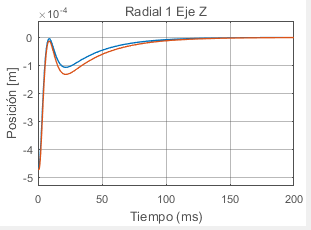
\includegraphics[width=\textwidth]{images/Capitulo_4/continuo_vs_discreto/radial_1_eje_z}
        \caption{Radial $1$.}
        %\label{fig:rmr:diagrama-de-polos}
    \end{subfigure}
    ~ %add desired spacing between images, e. g. ~, \quad, \qquad, \hfill etc. 
      %(or a blank line to force the subfigure onto a new line)
    \begin{subfigure}[b]{0.45\textwidth}
        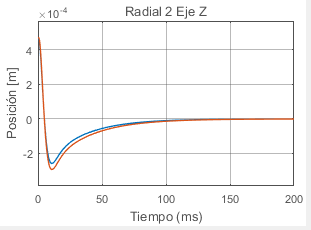
\includegraphics[width=\textwidth]{images/Capitulo_4/continuo_vs_discreto/radial_2_eje_z}
        \caption{Radial $2$.}
        %\label{fig:rmr:diagrama-de-fuerzas}
    \end{subfigure}
    \caption{Salida del sistema: Eje $Z$. Control integral continuo (azul) y control integral discreto (rojo).}
    \label{fig:Controlador_continuo_vs_Controlador_discreto_Eje_Z}
\end{figure}

\begin{figure}[H]
    \centering
    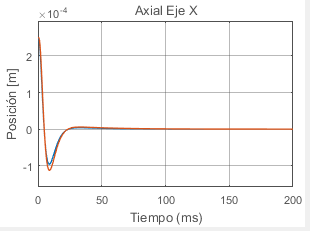
\includegraphics[width=0.45\textwidth]{images/Capitulo_4/continuo_vs_discreto/axial_eje_x}
    \caption{Salida del sistema: Eje axial $X$. Control integral continuo(azul) y control integral discreto (rojo).}
    \label{fig:Controlador_continuo_vs_Controlador_discreto_Eje_X}
\end{figure}


En las figuras \ref{fig:Controlador_continuo_vs_Controlador_discreto_Eje_Y}, \ref{fig:Controlador_continuo_vs_Controlador_discreto_Eje_Z} y \ref{fig:Controlador_continuo_vs_Controlador_discreto_Eje_X} podemos observar que ambos controladores se comportan de manera similar, validando que el controlador discreto emula correctamente al continuo.

\newpage

\section{Controlador calendarizado}

Esta simulaci�n consiste en un controlador integral discreto (figura \ref{fig:esquema-controlador-discreto}) y en un controlador integral discreto calendarizado (figura \ref{fig:esquema-controlador-calendarizado}), el controlador integral discreto fue linealizado en $\omega_s = 10000 \frac{rad}{s}$. Estos operan con una frecuencia de muestreo de $10kHz$. Esta simulaci�n se realiza sin cargas externas, primero con un $\omega_s = 10000$, y despu�s con un $\omega_s = -30000 \frac{rad}{s}$, con las condiciones iniciales:

\begin{table}[htb]
\centering
\begin{tabular}{|l|l|l|l|l|l|l|l|l|l|}
\hline
$x_c$     & $y_c$      & $z_c$     & $\dot{x}_c$     & $\dot{y}_c$     & $\dot{z}_c$     & $\phi$       & $\theta$    & $\dot{\phi}$     & $\dot{\theta}$   \\ \hline
$0.25 mm$ & $-0.25 mm$ & $0.25 mm$ & $0\frac{mm}{s}$ & $0\frac{mm}{s}$ & $0\frac{mm}{s}$ & $-0.0015rad$ & $0.0015rad$ & $0\frac{rad}{s}$ & $0\frac{rad}{s}$ \\ \hline
\end{tabular}
\caption{Condiciones Iniciales: Controlador integral discreto y Controlador integral discreto calendarizado.}
\end{table}

\begin{figure}[htb]
    \centering
    \begin{subfigure}[b]{0.45\textwidth}
        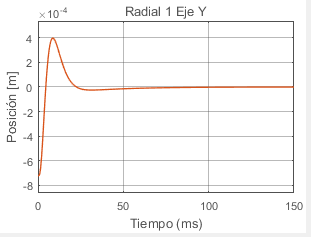
\includegraphics[width=\textwidth]{images/Capitulo_4/calendarizado_vs_normal/ws_10000/radial_1_eje_y}
        \caption{Radial $1$.}
        %\label{fig:rmr:diagrama-de-polos}
    \end{subfigure}
    ~ %add desired spacing between images, e. g. ~, \quad, \qquad, \hfill etc. 
      %(or a blank line to force the subfigure onto a new line)
    \begin{subfigure}[b]{0.45\textwidth}
        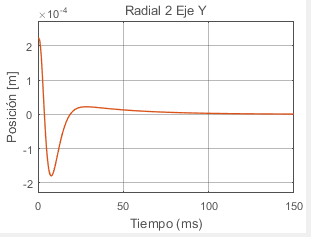
\includegraphics[width=\textwidth]{images/Capitulo_4/calendarizado_vs_normal/ws_10000/radial_2_eje_y}
        \caption{Radial $2$.}
        %\label{fig:rmr:diagrama-de-fuerzas}
    \end{subfigure}
    \caption{Salida del sistema: Eje $Y$. Control integral discreto (azul) y control integral discreto calendarizado (rojo), mostrando ambas curvas superpuestas en los gr�ficos. $\omega_s = 10000 \frac{rad}{s}$.}
    \label{fig:Controlador_linealizado_vs_Controlador_calendarizado_ws_10000_eje_y}
\end{figure}

\newpage

\begin{figure}[htb]
    \centering
    \begin{subfigure}[b]{0.45\textwidth}
        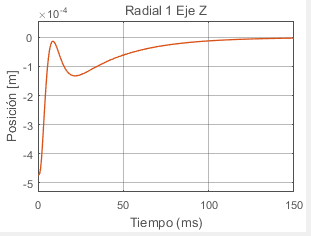
\includegraphics[width=\textwidth]{images/Capitulo_4/calendarizado_vs_normal/ws_10000/radial_1_eje_z}
        \caption{Radial $1$.}
        %\label{fig:rmr:diagrama-de-polos}
    \end{subfigure}
    ~ %add desired spacing between images, e. g. ~, \quad, \qquad, \hfill etc. 
      %(or a blank line to force the subfigure onto a new line)
    \begin{subfigure}[b]{0.45\textwidth}
        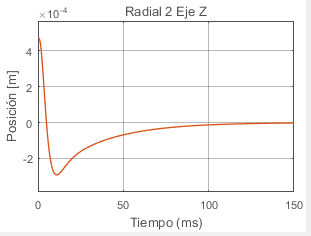
\includegraphics[width=\textwidth]{images/Capitulo_4/calendarizado_vs_normal/ws_10000/radial_2_eje_z}
        \caption{Radial $2$.}
        %\label{fig:rmr:diagrama-de-fuerzas}
    \end{subfigure}
    \caption{Salida del sistema: Eje $Z$. Control integral discreto (azul) y control integral discreto calendarizado (rojo), mostrando ambas curvas superpuestas en los gr�ficos. $\omega_s = 10000 \frac{rad}{s}$.}
    \label{fig:Controlador_linealizado_vs_Controlador_calendarizado_ws_10000_eje_z}
\end{figure}

\begin{figure}[H]
    \centering
    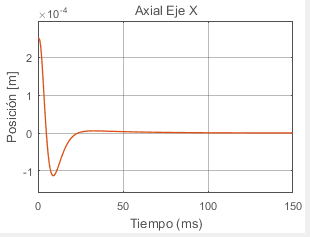
\includegraphics[width=0.45\textwidth]{images/Capitulo_4/calendarizado_vs_normal/ws_10000/axial_eje_x}
    \caption{Salida del sistema: Eje axial $X$. Control integral discreto (azul) y control integral discreto calendarizado (rojo), mostrando ambas curvas superpuestas en los gr�ficos. $\omega_s = 10000 \frac{rad}{s}$.}
    \label{fig:Controlador_linealizado_vs_Controlador_calendarizado_ws_10000_eje_x}
\end{figure}

Cuando la velocidad angular del rotor ($\omega_s$) es la misma que se us� durante el proceso de linealizaci�n, ambos controladores operan de la misma manera. Por lo tanto, tienen respuestas iguales, como se ilustra en las figuras \ref{fig:Controlador_linealizado_vs_Controlador_calendarizado_ws_10000_eje_y}, \ref{fig:Controlador_linealizado_vs_Controlador_calendarizado_ws_10000_eje_z}, \ref{fig:Controlador_linealizado_vs_Controlador_calendarizado_ws_10000_eje_x}.

\newpage

\begin{figure}[htb]
    \centering
    \begin{subfigure}[b]{0.45\textwidth}
        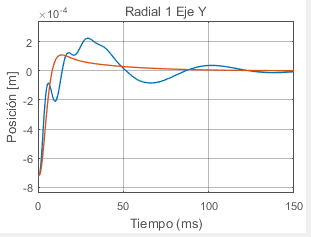
\includegraphics[width=\textwidth]{images/Capitulo_4/calendarizado_vs_normal/ws_30000/radial_1_eje_y}
        \caption{Radial $1$.}
        %\label{fig:rmr:diagrama-de-polos}
    \end{subfigure}
    ~ %add desired spacing between images, e. g. ~, \quad, \qquad, \hfill etc. 
      %(or a blank line to force the subfigure onto a new line)
    \begin{subfigure}[b]{0.45\textwidth}
        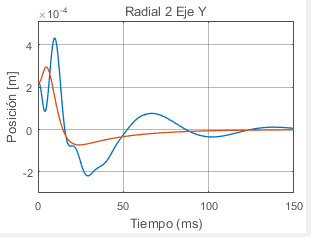
\includegraphics[width=\textwidth]{images/Capitulo_4/calendarizado_vs_normal/ws_30000/radial_2_eje_y}
        \caption{Radial $2$.}
        %\label{fig:rmr:diagrama-de-fuerzas}
    \end{subfigure}
    \caption{Salida del sistema: Eje $Y$. Control integral discreto (azul) y control integral discreto calendarizado (rojo). $\omega_s = -30000 \frac{rad}{s}$.}
    \label{fig:Controlador_linealizado_vs_Controlador_calendarizado_ws_30000_eje_y}
\end{figure}

\begin{figure}[htb]
    \centering
    \begin{subfigure}[b]{0.45\textwidth}
        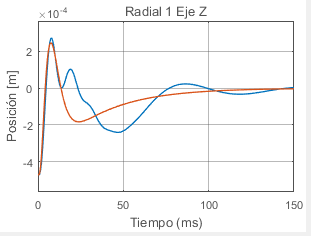
\includegraphics[width=\textwidth]{images/Capitulo_4/calendarizado_vs_normal/ws_30000/radial_1_eje_z}
        \caption{Radial $1$.}
        %\label{fig:rmr:diagrama-de-polos}
    \end{subfigure}
    ~ %add desired spacing between images, e. g. ~, \quad, \qquad, \hfill etc. 
      %(or a blank line to force the subfigure onto a new line)
    \begin{subfigure}[b]{0.45\textwidth}
        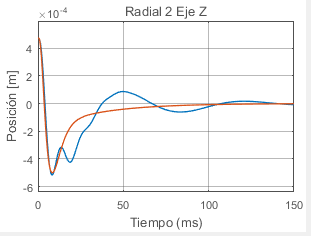
\includegraphics[width=\textwidth]{images/Capitulo_4/calendarizado_vs_normal/ws_30000/radial_2_eje_z}
        \caption{Radial $2$.}
        %\label{fig:rmr:diagrama-de-fuerzas}
    \end{subfigure}
    \caption{Salida del sistema: Eje $Z$. Control integral discreto (azul) y control integral discreto calendarizado (rojo). $\omega_s = -30000 \frac{rad}{s}$.}
    \label{fig:Controlador_linealizado_vs_Controlador_calendarizado_ws_30000_eje_z}
\end{figure}

\begin{figure}[htb]
    \centering
    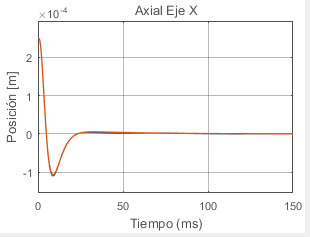
\includegraphics[width=0.45\textwidth]{images/Capitulo_4/calendarizado_vs_normal/ws_30000/axial_eje_x}
    \caption{Salida del sistema: Eje axial $X$. Control integral discreto (azul) y control integral discreto calendarizado (rojo). $\omega_s = -30000 \frac{rad}{s}$.}
    \label{fig:Controlador_linealizado_vs_Controlador_calendarizado_ws_30000_eje_x}
\end{figure}

\newpage

Cuando trabajan a velocidades angulares diferentes, el controlador no calendarizado presenta problemas para estabilizar el rotor debido a los efectos de la precesi�n. En cambio el control calendarizado no presenta problemas (fig. \ref{fig:Controlador_linealizado_vs_Controlador_calendarizado_ws_30000_eje_y}, \ref{fig:Controlador_linealizado_vs_Controlador_calendarizado_ws_30000_eje_z}, \ref{fig:Controlador_linealizado_vs_Controlador_calendarizado_ws_30000_eje_x}).  

\newpage

\section{Simulaci�n del accionamiento h�brido} 

Esta simulaci�n consiste en un controlador integral y observador discreto calendarizado con un $\omega_s = 10000 \frac{rad}{s}$ y con las condiciones iniciales:

\begin{table}[H]
\centering
\begin{tabular}{|l|l|l|l|l|l|l|l|l|l|}
\hline
$x_c$     & $y_c$      & $z_c$     & $\dot{x}_c$     & $\dot{y}_c$     & $\dot{z}_c$     & $\phi$       & $\theta$    & $\dot{\phi}$     & $\dot{\theta}$   \\ \hline
$0.1 mm$ & $-0.1 mm$ & $0.1 mm$ & $0\frac{mm}{s}$ & $0\frac{mm}{s}$ & $0\frac{mm}{s}$ & $-0.001rad$ & $0.001rad$ & $0\frac{rad}{s}$ & $0\frac{rad}{s}$ \\ \hline
\end{tabular}
\caption{Condiciones Iniciales: Accionamiento h�brido.}
\end{table}

Y con una fuerza aplicada en el centro de masa con valor de: 

\begin{table}[H]
\centering
\begin{tabular}{|l|l|l|}
\hline
\multicolumn{1}{|c|}{$F_{dx}$} & \multicolumn{1}{c|}{$F_{dy}$} & \multicolumn{1}{c|}{$F_{dz}$} \\ \hline
$sen(100\pi)[N]$               & $sen(200\pi)[N]$              & $3sen(200\pi) - 25 [N]$       \\ \hline
\end{tabular}
\end{table}

A diferencia de las simulaciones realizadas hasta ahora, la componente de fuerza $F_z$ del RMR es usada como se�al de control para el MCCE. A continuaci�n, se simulan dos casos: (a) con el MCCE descativado y (b) con el MCCE activado.


%\caption{Simulaci�n con carga combinada MCCE desactivado.}
%\label{fig:Simulacion_carga_combinada_MCCE_desactivado}


%\caption{Simulaci�n con carga combinada MCCE activado.}
%\label{fig:Simulacion_carga_combinada_MCCE_activada}


Se puede apreciar en la figura \ref{fig:Simulacion_carga_combinada_MCCE_desactivado} y \ref{fig:Simulacion_carga_combinada_MCCE_activada} que activar el lazo de control del MCCE no compromete la estabilidad del sistema. A continuaci�n se muestran los efectos en los electroimanes cuando se activa el MCCE. 


%\caption{Fuerzas ejercidas por los electroimanes (MCCE desactivado).}
%\label{fig:Simulacion_MCCE_desactivado}


%\caption{Fuerzas ejercidas por los electroimanes (MCCE activado).}
%\label{fig:Simulacion_MCCE_activado}


En el caso \textbf{(a)}, cuando el sistema se estabiliza, el MCCE mantiene una fuerza constante de $6 N$, mientras que el $RMR_z$ converge a una fuerza de $23 N$ (fig. \ref{fig:Simulacion_MCCE_desactivado}). En el caso \textbf{(b)}, la fuerza del MCCE converge a $29 N$, mientras que el $RMR_z$ converge a una fuerza aproximada de $0 N$  \ref{fig:Simulacion_MCCE_activado}).

En ambos casos, los controladores logran compensar las fuerzas combinadas que se les aplica y r�pidamente convergen al origen (fig. \ref{fig:Simulacion_MCCE_desactivado}, \ref{fig:Simulacion_MCCE_activado}).
